\begin{frame}{Trening}

	\begin{columns}
		\begin{column}{.7\hsize}

			\begin{table}[H]
				\centering
				\resizebox{\textwidth}{!}{%
				\begin{tabular}{|c|c|c|c|c|c|c|}
					\hline
					& \multicolumn{6}{c|}{Wynik bota po N-tym etapie treningu}\\
					Numer toru & po 1 etapie & po 2 etapie & po 3 etapie & po 4 etapie & po 5 etapie & po 6 etapie \\
					\hline
					\hline
					1 & 100\% & 100\% & 100\% & 100\% & 100\% & 100\% \\
					2 & 0\% & 33\% & 0\% & 33\% & 33\% & 100\% \\
					3 & 100\% & 100\% & 33\% & 100\% & 33\% & 100\% \\
					4 & 100\% & 100\% & 0\% & 100\% & 33\% & 100\% \\
					5 & 0\% & 33\% & 100\% & 100\% & 33\% & 100\% \\
					6 & 0\% & 0\% & 0\% & 33\% & 33\% & 66\% \\
					7 & 0\% & 0\% & 0\% & 0\% & 0\% & 66\% \\
					8 & 33\% & 0\% & 0\% & 0\% & 0\% & 33\% \\
					\hline
				\end{tabular}}
			\end{table}

		\end{column}
		\begin{column}{.4\hsize}
			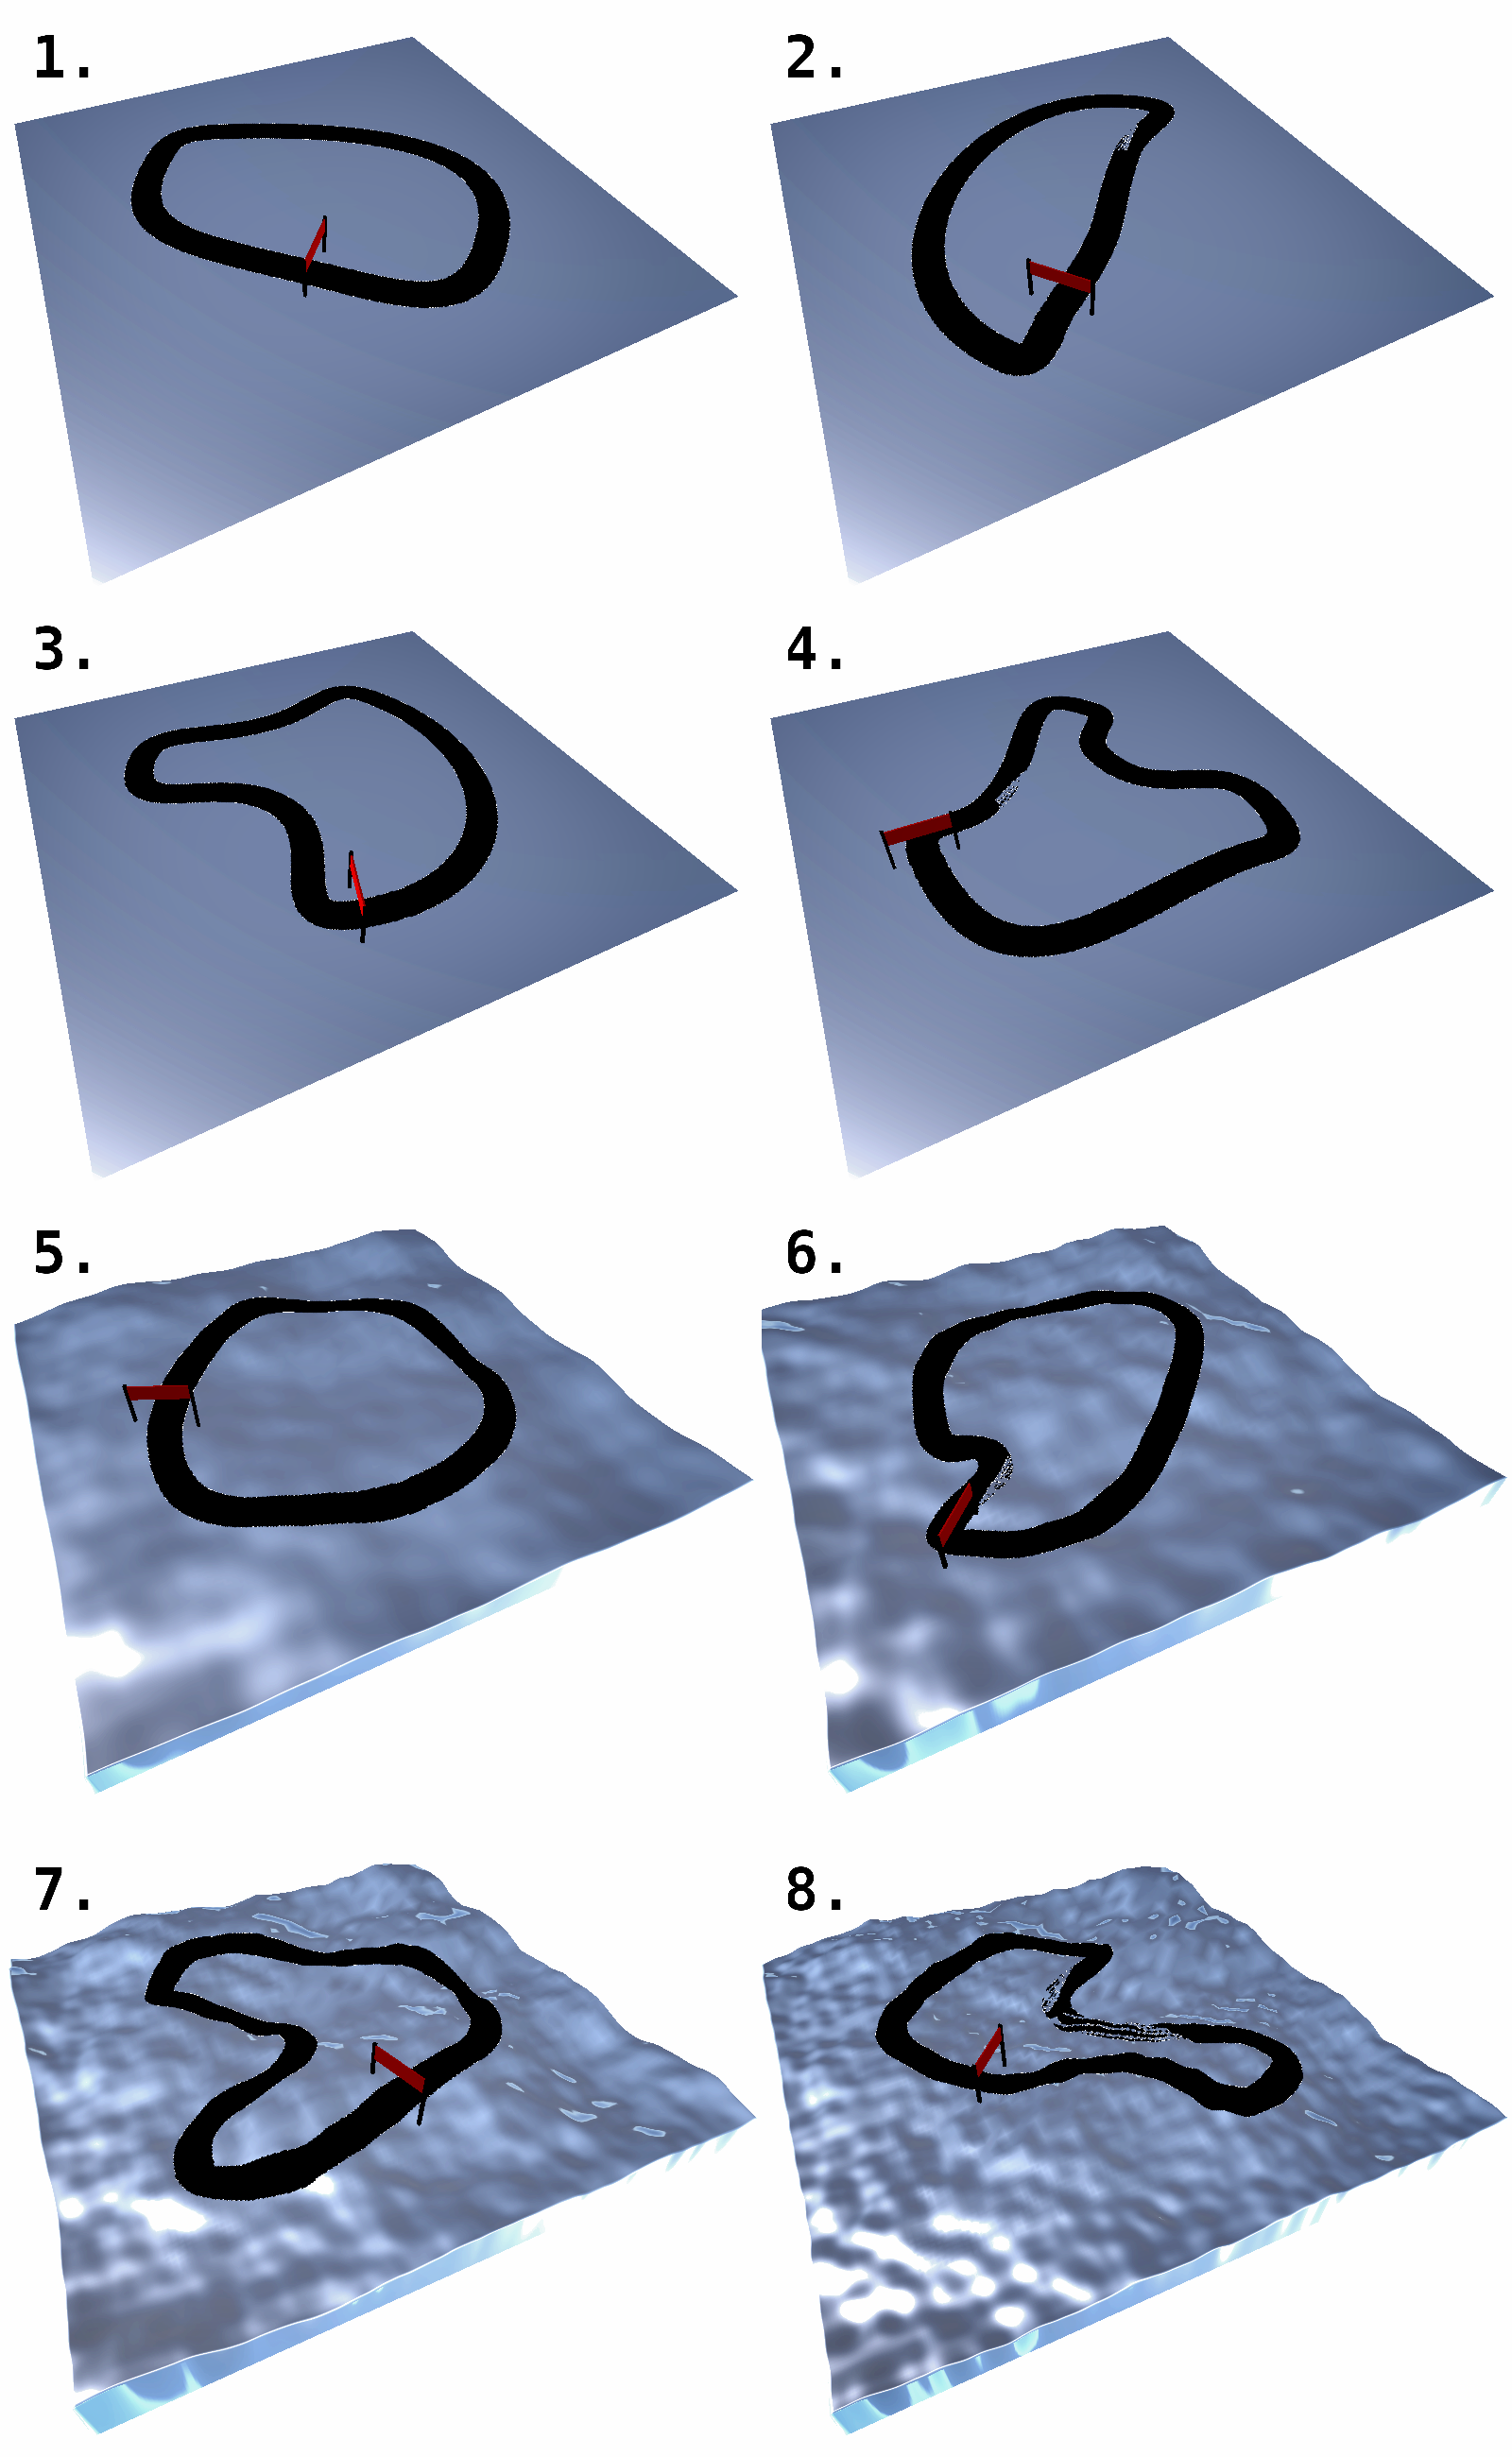
\includegraphics[width=\linewidth]{figures/trening_environs.png}
		\end{column}
	\end{columns}

\end{frame}
